
%
%  $Description: Author guidelines and sample document in LaTeX 2.09$
%
%  $Author: ienne $
%  $Date: 1995/09/15 15:20:59 $
%  $Revision: 1.4 $
%

%\documentclass[times, 10pt,twocolumn]{article}
\documentclass[conference]{IEEEtran}
%\usepackage{times}
\usepackage{graphicx}
%\usepackage{epsf}
%\usepackage{verbatim}
%\usepackage{psfig}
\usepackage{cite}
\usepackage{url}
%\usepackage{color}
\usepackage{alltt}
\usepackage{algorithm2e}

%\newcommand{\Fix}[1]{{\large\textbf{FIX}}#1{\large\textbf{FIX}}}
\newcommand{\Fix}[1]{#1}
\newcommand{\New}[1]{{\large\textbf{New}}#1{\large\textbf{New}}}
\newcommand{\Resolved}[1]{{\large\textbf{RESOLVED}}#1{\large\textbf{RESOLVED}}}

\newcommand{\realprojects}{a real project}
\newcommand{\Add}{\CodeIn{add}}
\newcommand{\AVTree}{\CodeIn{AVTree}}
\newcommand{\Assignment}[3]{$\langle$ \Object{#1}, \Object{#2}, \Object{#3} $\rangle$}
\newcommand{\BinaryTreeRemove}{\CodeIn{BinaryTree\_remove}}
\newcommand{\BinaryTree}{\CodeIn{BinaryTree}}
\newcommand{\Caption}{\caption}
\newcommand{\Char}[1]{`#1'}
\newcommand{\CheckRep}{\CodeIn{checkRep}}
\newcommand{\ClassC}{\CodeIn{C}}
\newcommand{\CodeIn}[1]{{\small\texttt{#1}}}
\newcommand{\CodeOutSize}{\scriptsize}
\newcommand{\Comment}[1]{}
\newcommand{\Ensures}{\CodeIn{ensures}}
\newcommand{\ExtractMax}{\CodeIn{extractMax}}
\newcommand{\FAL}{field-ordering}
\newcommand{\FALs}{field-orderings}
\newcommand{\Fact}{observation}
\newcommand{\Get}{\CodeIn{get}}
\newcommand{\HashSet}{\CodeIn{HashSet}}
\newcommand{\HeapArray}{\CodeIn{HeapArray}}
\newcommand{\Intro}[1]{\emph{#1}}
\newcommand{\Invariant}{\CodeIn{invariant}}
\newcommand{\JUC}{\CodeIn{java.\-util.\-Collections}}
\newcommand{\JUS}{\CodeIn{java.\-util.\-Set}}
\newcommand{\JUTM}{\CodeIn{java.\-util.\-TreeMap}}
\newcommand{\JUTS}{\CodeIn{java.\-util.\-TreeSet}}
\newcommand{\JUV}{\CodeIn{java.\-util.\-Vector}}
\newcommand{\JMLPlusJUnit}{JML+JUnit}
\newcommand{\Korat}{Korat}
\newcommand{\Left}{\CodeIn{left}}
\newcommand{\Lookup}{\CodeIn{lookup}}
\newcommand{\MethM}{\CodeIn{m}}
\newcommand{\Node}[1]{\CodeIn{N}$_#1$}
\newcommand{\Null}{\CodeIn{null}}
\newcommand{\Object}[1]{\CodeIn{o}\ensuremath{_#1}}
\newcommand{\PostM}{\MethM$_{post}$}
\newcommand{\PreM}{\MethM$_{pre}$}
\newcommand{\Put}{\CodeIn{put}}
\newcommand{\Remove}{\CodeIn{remove}}
\newcommand{\RepOk}{\CodeIn{repOk}}
\newcommand{\Requires}{\CodeIn{requires}}
\newcommand{\Reverse}{\CodeIn{reverse}}
\newcommand{\Right}{\CodeIn{right}}
\newcommand{\Root}{\CodeIn{root}}
\newcommand{\Set}{\CodeIn{set}}
\newcommand{\State}[1]{2^{#1}}
\newcommand{\TestEra}{TestEra}
\newcommand{\TreeMap}{\CodeIn{TreeMap}}

%\newenvironment{CodeOut}{\begin{scriptsize}}{\end{scriptsize}}
%\newenvironment{CodeOut}{\begin{scriptsize}}{\end{scriptsize}}
\newenvironment{CodeOut}{\begin{small}}{\end{small}}
\newenvironment{SmallOut}{\begin{small}}{\end{small}}

\newcommand{\pairwiseEquals}{PairwiseEquals}
\newcommand{\monitorEquals}{MonitorEquals}
%\newcommand{\monitorWField}{WholeStateW}
\newcommand{\traverseField}{WholeState}
\newcommand{\monitorSMSeq}{ModifyingSeq}
\newcommand{\monitorSeq}{WholeSeq}

\newcommand{\IntStack}{\CodeIn{IntStack}}
\newcommand{\UBStack}{\CodeIn{UBStack}}
\newcommand{\BSet}{\CodeIn{BSet}}
\newcommand{\BBag}{\CodeIn{BBag}}
\newcommand{\ShoppingCart}{\CodeIn{ShoppingCart}}
\newcommand{\BankAccount}{\CodeIn{BankAccount}}
\newcommand{\BinarySearchTree}{\CodeIn{BinarySearchTree}}
\newcommand{\LinkedList}{\CodeIn{LinkedList}}

\newcommand{\Book}{\CodeIn{Book}}
\newcommand{\Library}{\CodeIn{Library}}

\newcommand{\Jtest}{Jtest}
\newcommand{\JCrasher}{JCrasher}
\newcommand{\Daikon}{Daikon}
\newcommand{\JUnit}{JUnit}

\newcommand{\trie}{trie}

\newcommand{\Perl}{Perl}


\newcommand{\SubjectCount}{11}
\newcommand{\DSSubjectCount}{two}

\newcommand{\Equals}{\CodeIn{equals}}
\newcommand{\Pairwise}{PairwiseEquals}
\newcommand{\Subgraph}{MonitorEquals}
\newcommand{\Concrete}{WholeState}
\newcommand{\ModSeq}{ModifyingSeq}
\newcommand{\Seq}{WholeSeq}
\newcommand{\Aeq}{equality}

\newcommand{\Meaning}[1]{\ensuremath{[\![}#1\ensuremath{]\!]}}
\newcommand{\Pair}[2]{\ensuremath{\langle #1, #2 \rangle}}
\newcommand{\Triple}[3]{\ensuremath{\langle #1, #2, #3 \rangle}}
\newcommand{\SetSuch}[2]{\ensuremath{\{ #1 | #2 \}}}
%\newtheorem{definition}{Definition}
%\newtheorem{theorem}[definition]{Theorem}
\newcommand{\Equiv}[2]{\ensuremath{#1 \EquivSTRel{} #2}}
\newcommand{\EquivME}{\Equiv}
\newcommand{\EquivST}{\Equiv}
\newcommand{\EquivSTRel}{\ensuremath{\cong}}
\newcommand{\Redundant}[2]{\ensuremath{#1 \lhd #2}}
\newcommand{\VB}{\ensuremath{\mid}}
\newcommand{\MES}{method-entry state}

\newcommand{\SmallSpace}{\vspace*{-1.5ex}}
\newcommand{\Item}{\SmallSpace\item}
\newenvironment{Itemize}{\begin{itemize}}{\end{itemize}\SmallSpace}
\newenvironment{Enumerate}{\begin{enumerate}}{\end{enumerate}\SmallSpace}


\newcommand{\Small}[1]{{\small{#1}}}

\newcommand{\CenterCell}[1]{\multicolumn{1}{c|}{#1}}

%\usepackage{latex8}
%\usepackage{times}

%\documentstyle[times,art10,twocolumn,latex8]{article}

%-------------------------------------------------------------------------
% take the % away on next line to produce the final camera-ready version
\pagestyle{empty}

%-------------------------------------------------------------------------
\begin{document}

\title{SpotWeb: Detecting Framework Hotspots and Coldspots via Mining Open Source Code on the Web}

\author{Suresh Thummalapenta\\
Department of Computer Science\\ North Carolina State University \\
Raleigh, USA\\ sthumma@ncsu.edu\\
% For a paper whose authors are all at the same institution,
% omit the following lines up until the closing ``}''.
% Additional authors and addresses can be added with ``\and'',
% just like the second author.
\and
Tao Xie\\
Department of Computer Science\\ North Carolina State University \\
Raleigh, USA\\ xie@csc.ncsu.edu\\
}

\maketitle
\thispagestyle{empty}

\begin{abstract}

Software developers often face
challenges in reusing open source frameworks due to several factors
such as the framework complexity and lack of proper
documentation. In this paper, we propose a code-search-engine-based
approach that detects \Intro{hotspots} in a given framework
by mining code examples gathered from open source repositories available on the web; 
these hotspots are API classes and methods that are frequently reused. 
Hotspots can serve as starting points for developers
in understanding and reusing the given framework. 
Our approach also detects \Intro{coldspots}, which are API classes and methods that are rarely used.
Coldspots serve as caveats for developers as there can 
be difficulties in finding relevant code examples and are generally less exercised
compared to hotspots. We developed a tool, called SpotWeb, for
frameworks or libraries written in Java and used our tool
to detect hotspots and coldspots of eight widely used open source
frameworks. We show the utility of our detected hotspots 
by comparing these hotspots with the API classes reused by a real application
and compare our results with the results of a previous related approach.
\end{abstract}

\section {Introduction}

Reuse of existing open source frameworks or libraries (referred as frameworks)
has become a common practice in the
current software development process due to several factors such as low
cost and high efficiency. However, existing frameworks often offer
complex API methods that pose challenges to developers for effective reuse.
This complexity also makes the documentation of the framework a
vital resource. However, the documentation is often missing for many
existing frameworks and even if such documentation exists, it
is often outdated~\cite{document:leth}.

In general, frameworks expose certain areas (API classes and methods) of
flexibility that are intended for reuse by their users. Software
developers who reuse classes and methods of these frameworks must be aware of
these flexible areas for effective reuse of frameworks. These
areas of flexibility are often referred as \Intro{hotspots}.
As described by Pree~\cite{pree:metapatterns}, hotspots depict a framework's
flexibility and proneness to reuse. The foundations of hotspots are
built upon the Open-Closed principle by Martin~\cite{martin:open}.
The Open-Closed principle encompasses two main definitions: the
``open'' and the ``closed'' parts. The ``open'' parts (referred as \Intro{hooks}) represent
areas that are flexible and variant, whereas the ``closed'' parts (referred as \Intro{templates}) 
represent areas that are immutable in the given framework. 
A \Intro{hotspot} is defined as a combination of templates and hooks.

Hotspots are useful to both users and developers of the framework
in several ways. First, new users can browse and inspect hotspots to understand commonly
reused classes and find out the classes that the users want to reuse.
Second, users may have more confidence or tendencies in
reusing hotspots because generally bugs in these hotspots may be
fewer (or more easily exposed previously) than the ones in
non-hotspots; we can view the application code that reuses framework hotspots to be a special
type of test code that can help expose bugs in
hotspots. Third, developers or maintainers of these frameworks can choose to
invest their improvement effort (e.g., performance improvement or bug fixing) 
on these hotspots because the resulting returns on
investment may be substantial.

In contrast to hotspots, we call a framework's areas that
are rarely used by users as \Intro{coldspots}.
The concept of coldspots is introduced by our approach and these
coldspots can serve as caveats to users of the given framework.
As coldspots represent the rarely used classes and methods, there can be difficulties
in identifying relevant code examples that can help users in reusing
those classes and methods. Moreover, coldspots are generally less tested compared to hotspots
with regards to the ``testing'' conducted by API client code as
test code.

Detecting hotspots and coldspots of an input framework requires domain knowledge of how the API classes
and methods of the input framework are reused by applications, referred as client
applications. Various open source projects that reuse classes of a given input framework
are available on the web and these open source projects
can serve as a basis for gathering the information of how classes of the
input framework are reused, and hence can help in detecting hotspots and coldspots.
Therefore, our approach, called SpotWeb, leverages a code search engine (CSE) to gather
relevant code examples of classes of the input framework from these open source
projects. Given a query, a CSE can extract code examples
with usages of the query from open source projects available on the web. Our approach analyzes
gathered code examples statically and detects hotspots and coldspots of the
given framework. Our approach tackles
the problems related to the quality of code examples gathered
from a CSE by capturing the most common usages of classes through mining.

The paper\footnote{An earlier version of this work is described in a position paper
presented at MSR 2008~\cite{thummalapenta08:spotweb}.}makes the following main contributions:
\vspace{2ex}
\begin{Itemize}

\Item An approach for detecting hotspots of a given framework by analyzing relevant
code examples gathered from a CSE.
\vspace{3ex}
\Item An approach for detecting coldspots of a given framework.
\vspace{2ex}
\Item A tool (as an Eclipse plugin) implemented for the proposed approach 
and several evaluations to assess the effectiveness of the tool. In our evaluation,
SpotWeb detects hotspots and coldspots of eight widely used open source frameworks
by analyzing a total of $7.9$ million lines of code. We show the utility of 
detected hotspots by comparing detected hotspots
of a framework with a real application reusing that framework. We also compare our
results with the results of a previous related approach by Viljamaa~\cite{viljamaa:reverse}.
\end{Itemize}
\vspace{2ex}

The rest of the paper is organized as follows. 
Section~\ref{sec:example} explains our approach through an illustrative example.
Section~\ref{sec:specapproach} describes key aspects of the approach.
Section~\ref{sec:implementation} presents implementation details.
Section~\ref{sec:eval} discusses evaluation results.
Section~\ref{sec:threats} presents threats to validity.
\Comment{Section~\ref{sec:discussion} presents limitations and future work.}
Section~\ref{sec:related} presents related work.
Finally, Section~\ref{sec:conclusion} concludes.

\section{Example}
\label{sec:example}

\begin{figure*}[t]
\centering
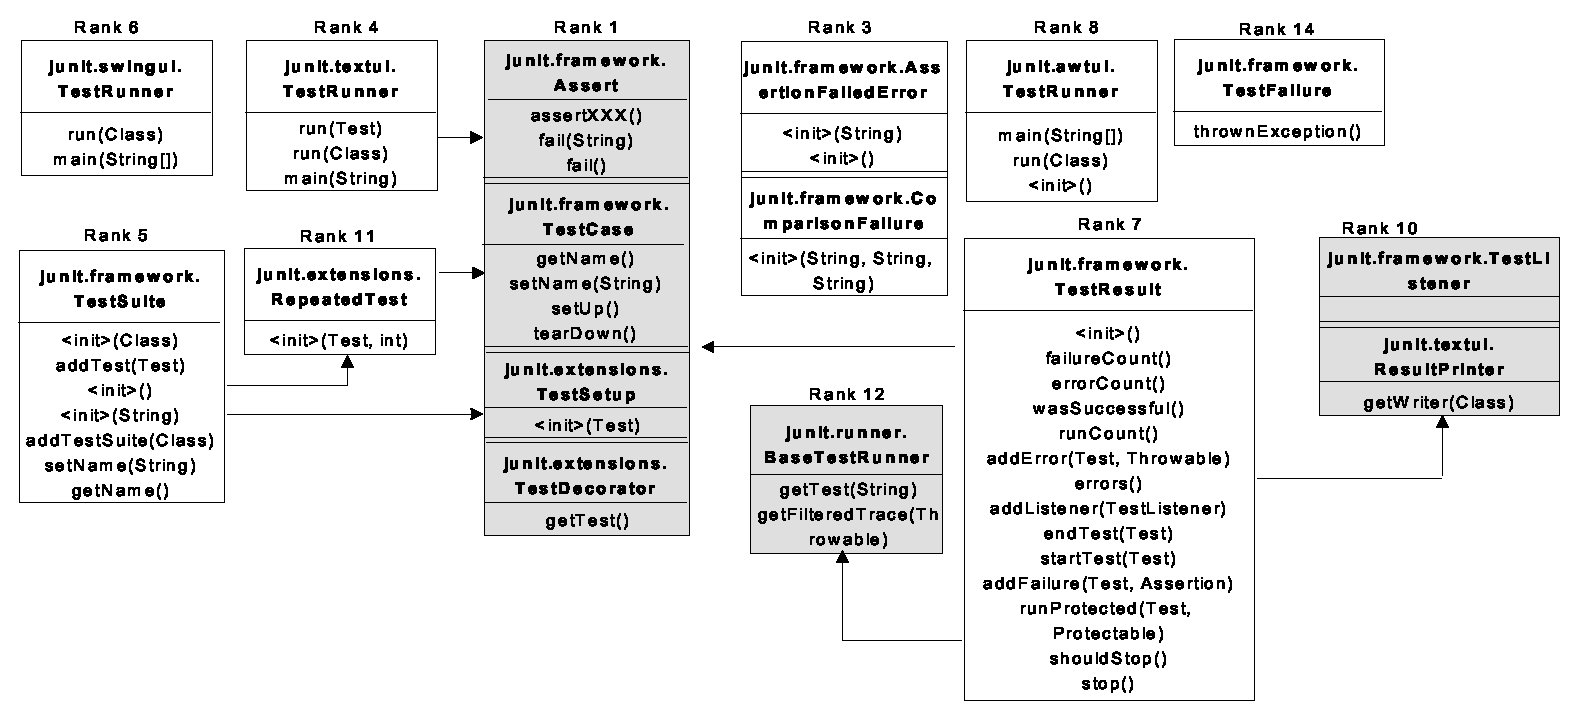
\includegraphics[scale=0.68,clip]{examplehotspot_final.eps}
\caption{Hotspot hierarchies identified for the JUnit framework} \label{fig:hotspotexample}
\end{figure*}

We next use an example to explain our approach and show how the detected
hotspots and coldspots can be used by the framework users. We use JUnit~\cite{JUNIT}, the
\emph{de facto} standard unit testing framework for Java, 
as an illustrative example for explaining our approach.

SpotWeb accepts an input framework, say JUnit, and extracts
\emph{FrameworkInfo} from the framework. The
\emph{FrameworkInfo} includes all classes, all interfaces, public
or protected methods of each class and interface, and inheritance
hierarchy among classes or interfaces of the framework. SpotWeb also captures
the constants defined by the input framework. SpotWeb
constructs different queries for each class or interface and
interacts with a CSE such as Google code search~\cite{GCSE} to
gather relevant code examples from existing open source projects that
reuse the classes of the input framework. For example, SpotWeb constructs
a query such as ``\CodeIn{lang:java junit.framework.TestSuite}'' for
gathering relevant code examples of the \CodeIn{TestSuite} class. These
gathered code examples are referred as a \emph{LocalRepository} for
the input framework. SpotWeb analyzes gathered code examples
statically and computes \emph{UsageMetrics} for classes, interfaces,
and public or protected methods of all classes and interfaces. For
example, the \emph{UsageMetrics} computed for the \CodeIn{TestSuite}
class show that the class is instantiated for 165 times and is
extended for 32 times. Similarly, the \emph{UsageMetrics} computed
for the method \CodeIn{addTest} of the \CodeIn{TestSuite} class show
that the method is invoked for 95 times. SpotWeb also gathers code
examples for each class or method and stores these code examples in
a repository, referred as \emph{ExampleDB}. Then SpotWeb uses the
algorithm shown in Figure~\ref{alg:hotspotalgo} for detecting
hotspots from the computed \emph{UsageMetrics}.

Initially, SpotWeb ranks methods in a non-ascending order based on
their \emph{UsageMetrics} and uses a threshold percentage $HT$ to
detect hotspot methods: the methods in the top $HT$ percentage with
a non-zero \emph{UsageMetrics} are detected as hotspot methods. 
The detected hotspot methods are then
grouped into their declaring classes, detected as hotspot classes.
These hotspot classes are ranked based on the minimum rank of the
hotspot methods declared by these classes. SpotWeb classifies the
hotspot classes into two categories (templates and hooks) based on
heuristics described in Step 4 of the algorithm shown in Figure~\ref{alg:hotspotalgo}. The hotspot classes of each
category are further grouped into hierarchies based on their
inheritance relationships. For example, SpotWeb detected classes
\CodeIn{Assert} and \CodeIn{TestCase} as hook hotspots in the JUnit
framework. As \CodeIn{TestCase} class extends \CodeIn{Assert} class,
SpotWeb groups both the classes into the same hierarchy. SpotWeb
assigns a rank to each hierarchy based on the minimum rank of the
hotspot classes contained in the hierarchy. For example, consider
that the \CodeIn{Assert} class has Rank 1 and the \CodeIn{TestCase}
class has Rank 2, and then the grouped hierarchy of the
\CodeIn{Assert} and \CodeIn{TestCase} classes is assigned with Rank
1. \Comment{The rank attribute uniquely identifies a hierarchy among all
other hierarchies.} Hierarchies with smaller ranks have higher preference
or importance to the hierarchies with larger ranks.

Figure~\ref{fig:hotspotexample} shows the hotspot hierarchies detected for the JUnit
framework. The figure also shows ranks assigned to each hierarchy.
\Comment{As the rank attribute uniquely identifies a hierarchy, we use the
rank as an identity for describing a hierarchy.}
Each hierarchy includes one or more hotspot classes and is shown as pairs of a class and its methods.
For example, Hierarchy 1 (hierarchy with Rank 1) has classes \CodeIn{Assert}, \CodeIn{TestCase}, \CodeIn{TestSetup},
and \CodeIn{TestDecorator}. We show template hierarchies in white and hook hierarchies in gray.
For example, Hierarchy 1 is a hook hierarchy and Hierarchy 3 is a template hierarchy.

Methods inside each class of a hierarchy are sorted
based on their computed \emph{UsageMetrics}. Sorting methods of a class
can assist the framework users in quickly identifying the methods that are often
used inside a given hotspot class. For example, consider the \CodeIn{TestSuite} class
shown in Hierarchy 5. The \CodeIn{TestSuite} class has three constructors \CodeIn{<init>(Class)},
\CodeIn{<init>()}, and \CodeIn{<init>(String)}. However, the \CodeIn{<init>(Class)} constructor
is often used compared to the other two constructors. Due to space limit,
we show all assertion methods such as \CodeIn{assertEquals} and \CodeIn{assertTrue}
of the class \CodeIn{Assert} of Hierarchy 1 as \CodeIn{assertXXX}.

The figure also displays dependencies among hotspot hierarchies 
(shown as arrows between hierarchies). \Comment{SpotWeb captures the
usage relationships among hotspot classes through dependencies.}
For example, Hierarchy $5$ has a
\CodeIn{TEMPLATE\_HOOK} dependency with Hierarchy $1$. This
dependency indicates that to reuse methods such as \CodeIn{addTest}
of the class \CodeIn{TestSuite} in Hierarchy 5, the user has to
define a new behavior for the classes in Hierarchy $1$ because the first argument
of \CodeIn{addTest} requires instances of classes such as \CodeIn{TestCase} of Hierarchy $1$.

\begin{figure}[t]
\begin{CodeOut}
\begin{alltt}
01:public class SRDAOTestCase 
02:\hspace*{0.4in}extends TestCase \{
03:\hspace*{0.1in}private SRDAO dao = null;...
04:\hspace*{0.1in}public SRDAOTestCase() \{
05:\hspace*{0.3in}super(); ... 
06:\hspace*{0.1in}\}
07:\hspace*{0.1in}protected void setUp() throws Exception \{
08:\hspace*{0.3in}...
09:\hspace*{0.3in}dao = (SRDAO)context.getBean("SRDAO");
10:\hspace*{0.3in}...
11:\hspace*{0.1in}\}
12:\hspace*{0.1in}public void tearDown() throws Exception \{
13:\hspace*{0.3in}dao = null; 
14:\hspace*{0.1in}\}
15:\hspace*{0.1in}public void testF() \{ ... \}
16:\hspace*{0.1in}public void testB() \{ ... \}
17:\hspace*{0.1in}...
18:\}
\end{alltt}
\end{CodeOut}
\Caption{\label{fig:hcodeexample} Suggested code example for the hook class \CodeIn{TestCase}.}
\begin{CodeOut}
\begin{alltt}
01:public class MyTestSuite \{ 
02:\hspace*{0.1in}...
03:\hspace*{0.1in}public static Test suite() \{
04:\hspace*{0.3in}TestSuite suite = new TestSuite("axis");
05:\hspace*{0.3in}suite.addTest(new SRDAOTestCase());
06:\hspace*{0.3in}return suite;
07:\hspace*{0.1in}\}
08:\hspace*{0.1in}...
09:\}
\end{alltt}
\end{CodeOut}
\Caption{\label{fig:tcodeexample} Suggested code example for the template class \CodeIn{TestSuite}.}\vspace{-2ex}
\end{figure}

We next describe how the hotspots detected by SpotWeb can be used by
the framework users to reuse classes of the JUnit framework. After reviewing
the hotspots shown in Figure~\ref{fig:hotspotexample}, consider that
a framework user wants to start with the method \CodeIn{addTest} of
the template class \CodeIn{TestSuite} in Hierarchy 5.
Figure~\ref{fig:hotspotexample} shows that Hierarchy 5 of the
\CodeIn{TestSuite} class has a \CodeIn{TEMPLATE\_HOOK} dependency
with the Hierarchy 1. This dependency indicates that the user may
need to define a new behavior for the associated hook hierarchy.
SpotWeb recommends the code example shown in
Figure~\ref{fig:hcodeexample} for the hook class \CodeIn{TestCase},
which is part of Hierarchy 1. The code example exhibits several
aspects that need to be handled by the user while extending the
\CodeIn{TestCase} class. For example, in the \CodeIn{setUp} method,
the user can write code for setting up the environment such as
instantiating necessary variables, and in the \CodeIn{tearDown}
method, the user can destroy the created variables. In addition, the code
example shows that names of the test methods in the extended class
of the \CodeIn{TestCase} class should start with the prefix \CodeIn{test}.
SpotWeb also recommends a code example for the \CodeIn{addTest} method and
the recommended code example is shown in
Figure~\ref{fig:tcodeexample}. The code example shows that the user
has to create an instance of the \CodeIn{TestSuite} class and then
add test cases through the \CodeIn{addTest} method.

An API class or method is identified as a coldspot if that class or method is neither
used directly nor used indirectly by gathered code examples. The complete
algorithm used for detecting coldspots is shown in Figure~\ref{alg:coldspotalg}. SpotWeb identified $20$
classes such as \CodeIn{Swapper}, \CodeIn{TestRunListener}, and \CodeIn{ExceptionTestCase} as coldspots
in the JUnit framework. However, coldspots are only suggestions
for users unfamiliar to that framework and SpotWeb does not intend to recommend users not to reuse
those coldspot classes. Sometimes, coldspots can also be helpful to
the framework developers in distributing their maintenance effort, because the framework
developers can give a low preference to the coldspot classes.

\section{Approach}
\label{sec:specapproach}
Our approach consists of five major components:
the framework reader, CSE, code downloader, code
analyzer, and spot builder. Figure~\ref{fig:architecture} shows an overview of all components
and flows among different components. We use JUnit
as an illustrative example for explaining our approach. 
\begin{figure}[t]
\centering
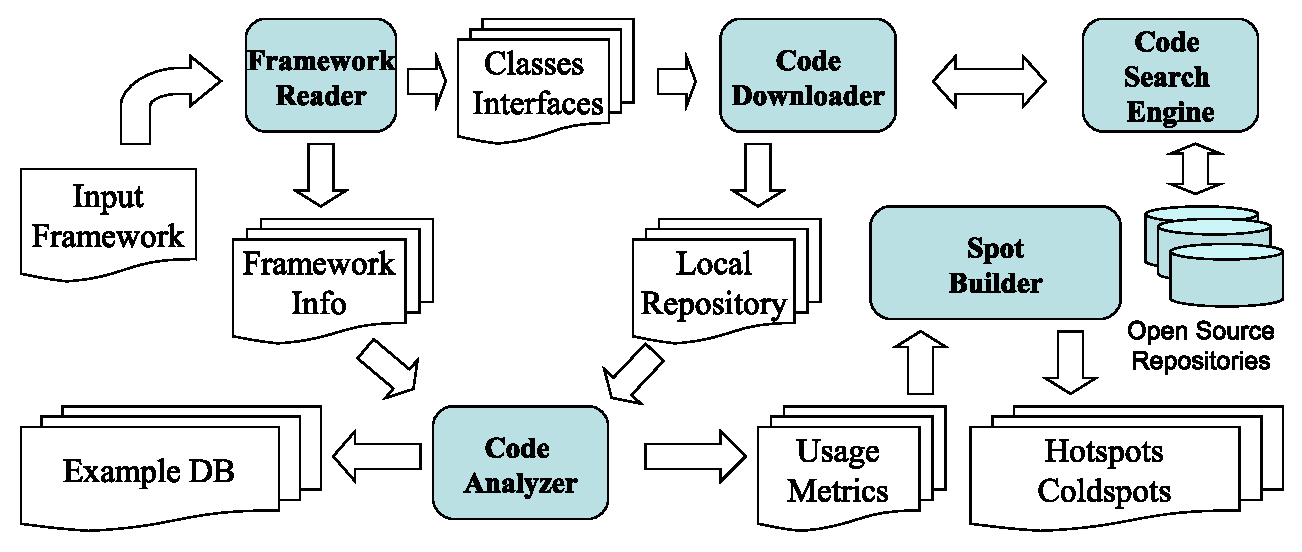
\includegraphics[scale=0.38,clip]{Framework_overview1.eps}
\caption{Overview of the SpotWeb approach} \label{fig:architecture}
\end{figure}
%--------------------------------------------------------------------------------
\subsection{Framework Reader} 
The framework reader component
takes a framework, say JUnit, as input and extracts the \emph{FrameworkInfo}
information. The \emph{FrameworkInfo} includes all classes, all interfaces, public
or protected methods of each class and interface.
%--------------------------------------------------------------------------------
\subsection{Code Downloader} 
The code downloader interacts with a CSE to download relevant code examples. 
For example, the code downloader constructs
a query such as ``\CodeIn{lang:java junit.framework.TestSuite}'' for
gathering relevant code examples of the \CodeIn{TestSuite} class.
The downloaded code examples, referred as \emph{LocalRepository}, are given as input
to the code analyzer. The code examples stored in the \emph{LocalRepository}
are often partial as CSE gathers individual source files,
instead of entire projects. In our approach, we used Google code search~\cite{GCSE}
for gathering relevant code code examples. There are two main reasons
for using Google code search as an underlying search engine in our approach: Google code search
provides open APIs to interact through client code and is well-maintained.

%--------------------------------------------------------------------------------
\subsection{Code Analyzer} 
The code analyzer analyzes code examples 
stored in the \emph{LocalRepository} statically and computes
\emph{UsageMetrics} for all classes, methods, exceptions, and constants of the input
framework. As these code examples are partial,
the code analyzer uses several type heuristics for resolving object types.
These type heuristics are described in our previous approach, called PARSEWeb~\cite{thummalapenta07:parseweb}.
The \emph{UsageMetrics} capture several ways of how often a class or an interface or a method 
of the input framework is used by gathered code examples.

The \emph{UsageMetrics} for a class include the
number of created instances (more precisely, the number of
constructor-call sites) and the number of times that the class is
extended. For an interface, the \emph{UsageMetrics} include the number
of times that the interface is implemented. We use notations
$IN_j$, $EX_j$, and $IM_j$ for the number of instances,
the number of extensions, and the number of implementations, respectively.
The consolidated usage metric $UM_j$ for a class or an interface 
is the sum of all the three preceding metrics. The \emph{UsageMetrics}
for an exception class include the number of times that the exception class
is used in the \CodeIn{catch} blocks or the \CodeIn{throw} statements. 

The code analyzer computes three types of \emph{UsageMetrics} for
methods: Invocations, Overrides, and Implements.
The \emph{Invocations} metric gives the number of times that the
method is invoked by the code examples. The \emph{Overrides} metric
gives the number of times that the method is overridden by the code
examples to define a new behavior. The \emph{Implements} metric,
specific for interfaces, gives the number of times that the method
is implemented. The code analyzer considers \CodeIn{static} methods as regular methods.
For constructors, the code analyzer computes only the \emph{Invocations} metric. 
We use notations $IN_i$, $OV_i$, and $IM_i$
for invocations, overrides, and implementations, respectively. 
The overall usage metric ($UM_i$) for a method is the sum of all the three
preceding metrics. 

The code analyzer identifies constants defined by the input framework through
the Java keywords such as \CodeIn{final} and \CodeIn{static}. The \emph{UsageMetrics}
for such a constant include the number of times that the constant is referred
by code examples gathered from CSE.

The code analyzer also gathers code examples for each class or method and 
stores these code examples in a repository, referred as \CodeIn{ExampleDB}. The \CodeIn{ExampleDB} is used
for recommending relevant code examples for a class or a method requested by the users. The relevant
code examples can further assist the users in making effective reuse of API classes and methods of the
input framework. 

\begin{figure}[t]
\begin{CodeOut}
Input: UsageMetrics of classes and methods, HT percentage\\
Output: Hotspot hierarchies and their dependencies\\
1:\emph{SortedMET} = Sort methods based on their usage metric values;\\
2:foreach \emph{$MET_i$} in $SortedMET$ \{\\
\hspace*{0.3in}if ($UM_i$ $\neq$ 0) \\
\hspace*{0.5in}if (Position of $MET_i$ $\leq$ ($HT$ * Size of $SortedMET$))\\
\hspace*{0.8in}Set $MET_i$ type as $HOTSPOT$; \\
%\hspace*{0.5in}else \\
%\hspace*{0.8in}Set $MET_i$ type as $WEAKSPOT$;\\ 
\hspace*{0.2in}\}\\
3:\{$C_1$, ... $C_n$\} = Group $HOTSPOT$ $MET_i$ based on their \\\hspace*{0.2in}declaring classes;\\
//Assign ranks to each $C_i$ and classify into templates and hooks\\
4:foreach \emph{$C_i$} in \{$C_1$, ... $C_n$\} \{\\
\hspace*{0.3in}Rank of $C_i$ = Minimum rank among all $MET_i$ of the $C_i$;\\
\hspace*{0.3in}if $C_i$ is an \emph{Interface} or \emph{Abstract class} or ($EX_i$ $>$ $IN_i$)\\
\hspace*{0.5in}Set type of $C_i$ to $HOOK$;\\
\hspace*{0.3in}otherwise\\ 
\hspace*{0.5in}Set type of $C_i$ to $TEMPLATE$;\\
\hspace*{0.2in}\}\\
5:Group $C_i$ of the same type into hierarchies based on inheritance;\\
6:Associate hook hierarchies to template hierarchies;\\
7:Define dependencies between template hierarchies;\\
8:Output hook and template hierarchies as hotspot hierarchies;\\
\end{CodeOut}
\caption{\small{Algorithm used for detecting hotspots through computed
\emph{UsageMetrics}}} \label{alg:hotspotalgo}
\end{figure}
%---------------------------------------------------------------------------------
\subsection{Spot Builder} 
The spot builder component (SBC) analyzes gathered code examples and detects 
hotspots and coldspots.
%---------------------------------------------------------------------------------
\subsubsection{Identification of hotspots}
The spot builder component (SBC) uses computed \emph{UsageMetrics} for
detecting hotspots. The algorithm used by SBC for detecting hotspots
is shown in Figure~\ref{alg:hotspotalgo}. We next describe the algorithm 
through an illustrative example shown in Figure~\ref{fig:frameworkex}. The figure
shows four classes $C_1$, $C_2$, $C_3$, and \CodeIn{ExceptClass}, and their declarations. 
The class $C_3$ is an \CodeIn{abstract} class. The \CodeIn{ExceptClass}
is an \CodeIn{Exception} class that can appear in exception-handling
constructs such as \CodeIn{catch} blocks. The figure also shows
computed usage metrics for each class, and its methods and constant variables. For example,
the class $C_1$ is instantiated for 10 times (shown as \CodeIn{IN}=10)
and the abstract class $C_3$ is extended for 12 times (shown as \CodeIn{EX}=12). 
The method $m_{2\_1}$ is invoked for 6 times and is overridden for 2 times.
Similarly, the constant \CodeIn{constC1} is accessed 6 times and the 
exception class \CodeIn{ExceptClass} is detected in \CodeIn{catch} blocks
for 9 times among gathered code examples.

\begin{figure}[t]
\centering
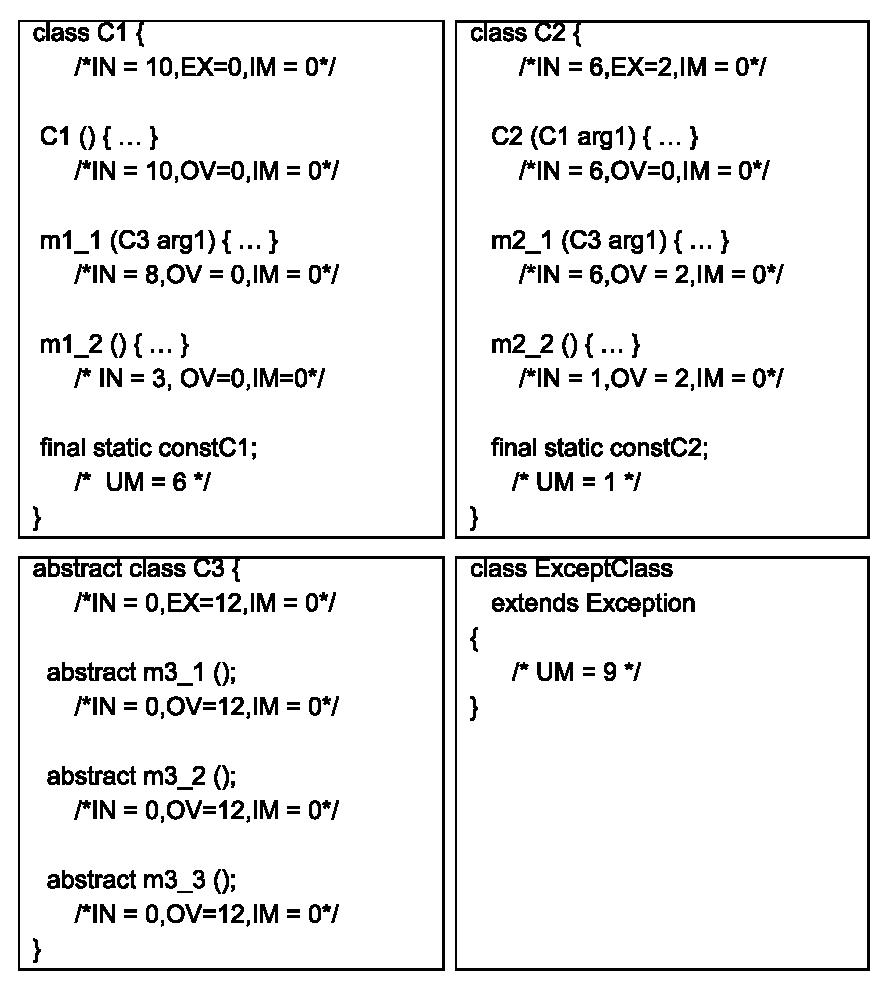
\includegraphics[scale=0.54,clip]{Approach_Example1.eps}
\caption{Example classes of a sample framework} \label{fig:frameworkex}
\end{figure}

Initially, SBC sorts $UM$ values of all methods, constants, and
exception classes. 
SBC uses a threshold percentage (referred as $HT$) and selects the
top $HT$ methods, whose usage metric is non-zero, as hotspot methods. For example, for a $HT$ of 45\%,
SBC identifies the methods such as $m_{3\_1}$, $m_{3\_2}$, $m_{3\_3}$, and $c_1$ as hotspot
methods. SBC groups the hotspot methods based on their declaring classes. 
The resulting classes are sorted based on the minimum rank among included hotspot methods in each class.
In the current example, the grouping process results in 
classes $C_3$ (methods: $m_{3\_1}$, $m_{3\_2}$, and $m_{3\_3}$), 
$C_1$ (methods: $c_1$ and $m_{1\_1}$), and $C_2$ (methods: $c_2$ and $m_{2\_1}$).
After grouping, SBC uses computed metrics of classes
to classify these classes further into templates and hooks. The criteria
used for classifying hotspot classes into templates and hooks are shown in Step 4 of the algorithm
shown in Figure~\ref{alg:hotspotalgo}. For the current example, 
SBC identifies class $C_3$ as a \CodeIn{HOOK} class, and classes
$C_1$ and $C_2$ as \CodeIn{TEMPLATE} classes. SBC further 
groups the classes of the same category based on their inheritance relationship. For example,
if $C_1$ has a parent class $P_1$ and both classes are classified as \CodeIn{TEMPLATE} classes,
SBC groups $C_1$ and $P_1$ into the same hierarchy.

SBC identifies dependencies among the detected hotspot hierarchies based on arguments
passed to methods of those classes. For example, if a template class, say X, has a constructor that requires
an instance of another template class, say Y, then SpotWeb captures
dependency of the form ``X $\rightarrow$ Y'', which describes that X
requires Y. SBC identifies two kinds of dependencies: \CodeIn{TEMPLATE\_HOOK}
and \CodeIn{TEMPLATE\_TEMPLATE}. A \CodeIn{TEMPLATE\_HOOK} dependency defines a relationship
between a template hierarchy and a hook hierarchy. SBC identifies that
a template hierarchy is dependent on a hook hierarchy if methods in the template
hierarchy types include some classes in the hook hierarchy as arguments. Such a dependency describes
that the users have to first define a new behavior for those related hook classes, say
extend the classes, and use the instances of those classes
as arguments. For example, SBC identifies that the class $C_1$ has a 
\CodeIn{TEMPLATE\_HOOK} dependency with 
the class $C_3$ as the method \CodeIn{$m_{1\_1}$} requires an instance of $C_3$ 
as an argument. Similarly, SBC identifies \CodeIn{TEMPLATE\_TEMPLATE}
hierarchies when one template hierarchy is dependent on another template hierarchy.
For example, the class $C_2$ has a \CodeIn{TEMPLATE\_TEMPLATE} dependency
with the class $C_1$. 

\Comment{
\begin{figure}[t]
\begin{CodeOut}
Input: A method $M_i$ of a class $C_j$\\
Output: Is the method a coldspot or not?\\
if ($UM_i$ $\neq$ 0) Return false;\\
if ($C_j$ is an interface) \{\\
\hspace*{0.3in}//verify all implemented methods of $M_i$\\
\hspace*{0.3in}if (All implemented methods of $M_i$ are coldspots) 
\hspace*{0.5in}Return true; \\
\hspace*{0.3in}else \\
\hspace*{0.5in}Return false; \}\\
if ($M_i$ is abstract) \{\\
\hspace*{0.3in}//Verify all overridden methods of $M_i$\\
\hspace*{0.3in}if (All overridden methods of $M_i$ are coldspots) 
\hspace*{0.5in}Return true; \\
\hspace*{0.3in}else \\
\hspace*{0.5in}Return false; \}\\
if (All callers of $M_i$ are coldspots) \\
\hspace*{0.3in}Return true; \\
else \\
\hspace*{0.3in}Return false;
\end{CodeOut}
\caption{\label{alg:coldspotalg}Algorithm for detecting whether a method is a coldspot.} 
\end{figure}}
\begin{figure}[t]
\begin{CodeOut}
Input: A method $M_i$ of a class $C_j$\\
Output: Is the method a coldspot or not?\\
1:Return false if the method is reused atleast once;\\
2:if $C_j$ is an interface \\
%\hspace*{0.3in}//verify all implemented methods of $M_i$\\
\hspace*{0.3in}Return true if all implemented methods of $M_i$ are coldspots; 
\hspace*{0.3in}Otherwise return false; \\
3:if $M_i$ is abstract \\
%\hspace*{0.3in}//Verify all overridden methods of $M_i$\\
\hspace*{0.3in}Return true if all overridden methods of $M_i$ are coldspots;
\hspace*{0.3in}Otherwise return false; \\
4:Return true if all callers of $M_i$ are coldspots \\
\hspace*{0.3in}Otherwise return false; \\
\end{CodeOut}
\caption{\label{alg:coldspotalg}Algorithm for detecting whether a method is a coldspot.} 
\end{figure}
%--------------------------------------------------------------------------
\subsubsection{Identification of coldspots}
SBC identifies classes and methods (of the input framework) that are rarely or never used
by gathered code examples as coldspots. However, detecting coldspots based on only the
\emph{UsageMetrics} can give many false positives. For example, the
\emph{UsageMetrics} for an abstract method defined in a class can be zero, as
gathered code examples refer to the concrete implementation provided
by some of the abstract classes's subclasses. In this case, this abstract method is
not a coldspot as the method is indirectly referenced through the
subclasses. Therefore, to reduce the number of false positives
while identifying coldspots, the code analyzer uses a recursive
algorithm shown in Figure~\ref{alg:coldspotalg}. 
\Comment{The \emph{UsageMetrics} referred by the algorithm is the sum of metrics
\emph{Invocations}, \emph{Overrides}, and \emph{Implements} computed
for a method. If computed \emph{UsageMetrics} are not zero, then
the method is identified not as a coldspot. If the current method
belongs to an interface, our algorithm recursively checks whether
all the corresponding methods in the implemented classes of the
input framework are also coldspots. If all of them are coldspots, the
code analyzer identifies the current method as a coldspot. The code
analyzer uses a similar approach when the method is abstract. If the
current method under analysis does not belong to any of the
preceding categories, the code analyzer checks whether all other
methods of the input framework that invoke the current method are also
coldspots.} Step 4 of the algorithm (related to callers)
is performed to identify indirect usages of a method of the input framework. 
SBC groups detected coldspot methods into their declaring classes.

%--------------------------------------------------------------------
\section{Implementation}
\label{sec:implementation}
\Fix{We developed SpotWeb as an Eclipse plugin. SpotWeb accepts an input framework in the form
of an Eclipse project. SpotWeb requires the input framework to be
compilable, i.e., all dependent jars have to be specified in
the classpath of the input framework. In the SpotWeb implementation, 
we used the $HT$ percentage of 15\%, which is derived based on our
initial empirical experience.}
%--------------------------------------------------------------------
\section {Evaluation}
\label{sec:eval}

We evaluated SpotWeb with eight widely used open source frameworks,
which differ in size and purpose. In our evaluation, we investigate the
following research questions. 

\begin{Itemize}
\item What is the percentage of hotspot and coldspot 
classes and methods among the total number of classes and methods in each framework, respectively? 
This research question helps to characterize the usages of a framework and 
effort in learning to reuse the framework. 
\item Is the subset of classes and methods detected
as hotspots indeed useful in helping effective framework reuse? We address the preceding question by 
showing that detected hotspots include classes and methods of a framework reused by a real application.
This evaluation helps to show that our approach can help reduce the effort
of users by suggesting a subset of classes and methods as hotspots.
\item What is the effectiveness of our hotspot detection in terms of precision and
recall? We address the preceding question through two evaluations. First, we compare
the detected hotspot classes with the classes described in the documentation associated
with the frameworks. Second, we compare the detected hotspot classes with 
the hotspots detected by a previous related approach by Viljamaa~\cite{viljamaa:reverse}.
\end{Itemize}

\vspace{1.5ex}
The subjects used in our evaluation and their
characteristics such as the number of classes and methods are shown
in Columns ``Classes'' and ``Methods'' of Table~\ref{tab:subjects}.
Column ``Samples'' of Table~\ref{tab:subjects} shows the number of
code examples gathered from Google code search~\cite{GCSE} and Column ``KLOC'' shows the total number of
kilo lines of Java code analyzed by SpotWeb for identifying hotspots
and coldspots. One of the major advantages of SpotWeb compared to
other approaches is the large number of analyzed code examples
that can help detect hotspots and coldspots effectively.

\setlength{\tabcolsep}{1pt}
\begin{table*}[t]
\begin{CodeOut}
\begin{center}
\centering \caption {\label{tab:subjects} Subjects used for evaluating SpotWeb.}
\begin {tabular} {|l|c|c|c|c|l|}
\hline
Subject&\# Classes&\# Methods&\# Samples&\# KLOC&\CenterCell{URL}\\
\hline Log4j&207&1543&9768&2064&logging.apache.org/log4j\\
\hline JUnit&56&531&8891&1558&www.junit.org\\
\hline JGraphT&177&931&289&30&jgrapht.sourceforge.net\\
\hline Grappa&44&561&2071&1978&www.graphviz.org\\
\hline OpenJGraph&210&1365&1076&113&openjgraph.sourceforge.net\\
\hline JUNG&461&3241&2390&353&jung.sourceforge.net\\
\hline BCEL&357&3048&5225&1219&jakarta.apache.org/bcel\\
\hline Javassit&249&2149&3226&631&www.csg.is.titech.ac.jp/chiba/javassist\\
\hline \textbf{TOTAL}&1761&13369&32936&7946&\\
\hline
\end{tabular}
\end{center}
\end{CodeOut}
\end{table*}
\Comment{%---------------------------------------------------------------------------------------------
\subsection{Subjects}
\label{sec:subjects}
Log4j is a library used for inserting
logs in source code. JUnit is the
\emph{de facto} standard unit testing framework for the Java
programming language. JGraphT, Grappa, OpenJGraph, and JUNG are four
graph libraries that provide several graph manipulation utilities.
BCEL and Javassit are libraries that provide functionality for
creating, analyzing, and manipulating Java class files.
}

\setlength{\tabcolsep}{1pt}
\begin{table*}[t]
\begin{CodeOut}
\begin{center}
\centering \caption {\label{tab:hotanddead} Evaluation results showing the
detected hotspots and coldspots.}
\begin {tabular} {|l|c|c|c|c|c|c|c|c|c|c|c|}
\hline
Subject&\# Classes&\multicolumn{5}{|c|}{Hotspot classes}&\multicolumn{2}{|c|}{Coldspot classes}&\multicolumn{3}{|c|}{Hotspot methods}\\
\cline{3-12}
&&\# Classes&\%&\# Templ&\# Hooks&\# Depend&\#Classes&\%&\# Total Methods&\# Hotspot Methods&\%\\
\hline Log4j        &207&56&27.05&35&11&22&131&63.28&1543&299&19.38\\
\hline JUnit            &56&14&25&8&3&7&22&39.28&531&77&14.50\\
\hline JGraphT      &177&41&23.16&20&8&0&135&76.27&931&102&10.96\\
\hline Grappa           &44&16&36.36&11&2&3&23&52.27&561&50&8.91\\
\hline OpenJGraph   &210&35&16.67&21&6&7&172&81.90&1365&76&5.57\\
\hline JUNG             &461&195&42.29&128&17&109&222&48.15&3241&569&17.55\\
\hline BCEL             &357&121&33.89&74&9&59&192&53.78&3048&580&19.03\\
\hline Javassit     &249&70&28.11&57&4&14&175&70.28&2149&371&17.26\\
\hline
\end{tabular}
\end{center}
\end{CodeOut}
\end{table*}
%---------------------------------------------------------------------------------------------
\subsection{Statistics of Hotspots and Coldspots}
\label{sec:hotspotsres}
We next address the first question on the percentage of classes and methods classified
as hotspots or coldspots. These statistics help identify the possibilities of reuse in a framework
and the amount of effort required by a new user in getting familiar with the given framework.
Table~\ref{tab:hotanddead} shows the statistics of hotspots in all frameworks.
Column ``Subject'' shows the name of the input framework. Columns ``Hotspot classes''
and ``Coldspot classes'' present the number of classes classified as hotspots and
coldspots, respectively. Column ``Hotspot methods'' shows the number of methods identified
as hotspot methods. Sub-columns ``Classes'' and ``\%'' of Column ``Hotspot classes'' show the number of hotspot classes
and their percentages among the total number of classes. Columns ``Templ'', ``Hooks'', and ``Depend''
give the number of template hierarchies, hook hierarchies, and their dependencies, respectively. Sub-columns
``Classes'' and ``\%'' of Column ``Coldspots'' show the number of coldspot classes and their percentages.

\begin{figure}[t]
\centering
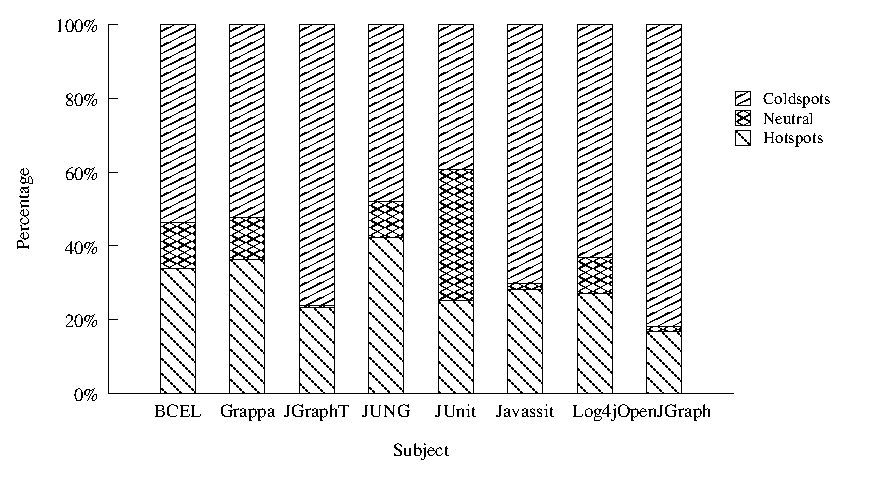
\includegraphics[scale=0.65,clip]{hotanddeadstats.eps}
\caption{\label{fig:hotdeadstats} Distribution of hotspot and coldspot percentages in all subject frameworks.} 
\end{figure}

Our results show that the percentage of hotspots for all subjects
ranges from 16\% to 42\%, whereas the percentage of coldspots ranges
from 39\% to 82\%. These statistics help characterize the effort in reusing 
a given framework. For example, the required effort for learning to reuse 
the JUnit framework can be low compared to the required effort for learning to reuse
the JUNG library because the number of hotspots of the JUNG library is
greater than the number of hotspots of the JUnit framework; these hotspots can 
often be browsed or investigated by the users to learn how to reuse the framework.
Figure~\ref{fig:hotdeadstats} presents the
distribution of hotspot and coldspot percentages of all subjects. 
The distribution chart shows that OpenJGraph and JGraphT frameworks
have the lowest percentage of hotspots and the highest percentage of
coldspots. This scenario can provide a hint that only a few classes of these
frameworks are often reused. In the figure, we also show a new classification called
``Neutral'', which represents classes that do not belong to either
the hotspot or coldspot category. The graph shows that the
percentage of classes in the Neutral category is relatively low for
all subjects except JUnit. This characteristic indicates that a class
is either reused heavily or is never reused, and only in a few cases
a class is occasionally reused.

We next describe a few example hotspot classes detected for the four graph libraries
JGraphT, Grappa, OpenJGraph, and Grappa. Each graph library provides several
different types of graphs. For example, the JUNG library provides 
graphs such as \CodeIn{DirectedGraph}, \CodeIn{ArchetypeGraph},
and \CodeIn{HyperGraph}.  SpotWeb identified the graph type that is commonly
used among all different types provided by each library. For example, SpotWeb
identified that graphs \CodeIn{DefaultListenableGraph}, \CodeIn{DirectedSparseGraph}, \CodeIn{DirectedGraphImpl},
and \CodeIn{Graph} are the commonly used graph types in JGraphT, JUNG, OpenJGraph, and Grappa
graph libraries, respectively. 
%----------------------------------------------------------------------------------------------
\subsection{Utilities of Hotspots}
\label{sec:hotspotuse}
We next try to address the second question on whether the subset of classes and methods
detected as hotspots is indeed useful in helping effective framework reuse. 
We use DNSJava\footnote{\url{http://www.dnsjava.org/}},
a popular framework that provides implementation of DNS in Java, as an input framework. 
We choose DNSJava for two primary reasons: DNSJava is used as a subject in several
previous approaches and the DNSJava webpage provides example applications that can be used to validate
the detected hotspots. We classify all DNSJava-reusing applications available on the web through Google code search
(except the James\footnote{\url{http://james.apache.org/}} 
application) as training applications for SpotWeb to detect 
hotspots of DNSJava. We validate the detected hotspots using James as a test application.
We selected James as the test application, because James is one of the example applications
described in the webpage of DNSJava.

\setlength{\tabcolsep}{1pt}
\begin{table}[t]
\begin{CodeOut}
\begin{center}
\centering \caption {\label{tab:jamesres} Hotspots of DNSJava reused by James.}
\begin {tabular} {|l|c|c|c|c|}
\hline
&James&SpotWeb&Precision&Recall\\
\hline Classes&17&16&32&94.11\\
\hline Methods&18&16&8.42&88.88\\
\hline Exceptions&1&1&33.33&100\\
\hline Constants&7&7&14&100\\
\hline
\end{tabular}
\end{center}
\end{CodeOut}\vspace{-2ex}
\end{table}

To show the utility of the detected hotspots, we identify the DNSJava classes 
and methods that are reused by James and compute the percentage of those classes detected
by SpotWeb. DNSJava includes 151 classes and 1224 methods. The
James application reused 17 classes and 18 methods of DNSJava. James also used 1 exception
class and 7 constants declared by DNSJava. \Fix{SpotWeb identified 47 classes, 190 methods, 3 exceptions,
and 50 constants as hotspots in DNSJava. Table~\ref{tab:jamesres} shows our evaluation results
in terms of precision and recall.

Column ``James'' shows the number of classes, 
methods, exceptions, and constants used by James. Column ``SpotWeb'' shows the
number of the ones (used by James) that are among detected hotspots by SpotWeb. 
The hotspots detected by SpotWeb include 16 classes and 16 methods reused by James. Moreover, SpotWeb also correctly
detected all 7 constants and 1 exception class referred by James. This evaluation shows that 
the subset of classes and methods detected as hotspots are 
indeed useful and can help reduce the effort of a programmer unfamiliar
to the framework.

SpotWeb could not detect one hotspot
class, called \CodeIn{Resolver}. The primary reason is that \CodeIn{Resolver} is an interface
and gathered code examples do not include any usages of the \CodeIn{Resolver} interface.
The results show that SpotWeb has a high recall and low precision with respect
to the James application. In our approach, we incline toward a high recall because
with a high recall, framework users would miss only few hotspot classes. We discuss
more on how we alleviate low precision in the subsequent evaluation.}
%---------------------------------------------------------------------------------------------
\subsection{Effectiveness of Hotspot Detection}
We next address the third question regarding the effectiveness of our hotspot detection
with respect to precision and recall through two evaluations. First, we compare
the detected hotspots of JUnit and Log4j frameworks with available documentations.
Second, we compare SpotWeb results with the results of a previous approach 
by Vijamaa~\cite{viljamaa:reverse}.

%---------------------------------------------------------------------------------------------
\subsubsection{Comparison with documentation}
\label{sec:doccomp}
We next analyze the effectiveness of hotspot detection through the
evaluation results with Log4j and JUnit frameworks. The primary
reason for selecting Log4j\footnote{\url{http://logging.apache.org/log4j/docs/manual.html}}
and JUnit\footnote{\url{http://junit.sourceforge.net/doc/cookstour/cookstour.htm}}
for analysis is the availability of their documentation that can
help validate the detected hotspots. 

Log4j provides several features such as Appenders and Layouts, and
for each such feature Log4j provides several classes. For example, Log4j
provides classes \CodeIn{ConsoleAppender} and \CodeIn{JDBCAppender} for the appender feature.
Among those several classes provided for each feature, a few classes are
much more often used than other classes. The features described in the documentation of Log4j are shown in
Columns ``Feature'' and ``Description'' of Table~\ref{tab:hdresults}. Column
``Class'' shows the commonly used classes for each feature. Each of these
classes serves as starting points for using those features.

\setlength{\tabcolsep}{1pt}
\begin{table*}[t]
\begin{CodeOut}
\begin{center}
\centering \caption {\label{tab:hdresults} Hotspots described in the Log4j documentation.}
\begin {tabular} {|l|l|l|c|c|}
\hline
Feature&\CenterCell{Description}&\CenterCell{Class}&Rank&Type\\
\hline Loggers&Log the messages of several levels&Category&1&\CodeIn{TEMPLATE}\\
\hline &&Logger&9&\CodeIn{HOOK}\\
\hline &&Level&4&\CodeIn{HOOK}\\
\hline Appenders&Allows logging to multiple destinations&ConsoleAppender&11&\CodeIn{TEMPLATE}\\
\hline &&FileAppender&16&\CodeIn{TEMPLATE}\\
\hline Layouts&Helps to format the logging request&PatternLayout&5&\CodeIn{TEMPLATE}\\
\hline &&SimpleLayout&13&\CodeIn{TEMPLATE}\\
\hline Configurators&Helps to configure Log4j&BasicConfigurator&2&\CodeIn{TEMPLATE}\\
\hline &&PropertyConfigurator&3&\CodeIn{TEMPLATE}\\
\hline &&DOMConfigurator&7&\CodeIn{TEMPLATE}\\
\hline Loaders&Helps to load resources&Loader&27&\CodeIn{TEMPLATE}\\
\hline NDC&Nested diagnostic constant&NDC&12&\CodeIn{TEMPLATE}\\
\hline
\end{tabular}
\end{center}
\end{CodeOut}
\end{table*}

SpotWeb identified 56 classes as hotspots in Log4j for
the $HT$ percentage of 15\%, and these classes captured 
all 12 starting points described in the
documentation resulting in a recall of 100\%. In constrast, the
precision is 21.42\%.  Column ``Rank'' of Table~\ref{tab:hdresults} presents the rank 
of each documented class among the total number of 
hotspots detected by SpotWeb. Column ``Type'' shows
whether the detected hotspot is a \CodeIn{TEMPLATE} or a
\CodeIn{HOOK}. The table also shows that except the
\CodeIn{Loader} class, all other 11 hotspot classes are ranked among
the top 16 classes of the total 56 classes. Therefore, a user who
plans to reuse classes of Log4j can refer to the first 16
classes suggested by SpotWeb to identify where to start reusing the
framework.

We used the cookbook provided with the JUnit framework to verify the
detected hotspots. Hotspots detected in the JUnit framework are
shown in Figure~\ref{fig:hotspotexample}. SpotWeb identified 
5 out of 6 hotspot classes described in the cookbook resulting in a recall of
83.33\% and precision 35.71\%. 

\begin{figure*}[t]
\centering
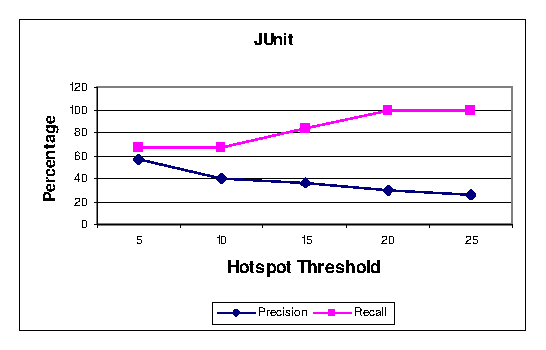
\includegraphics[scale=0.72,clip]{junit.eps}
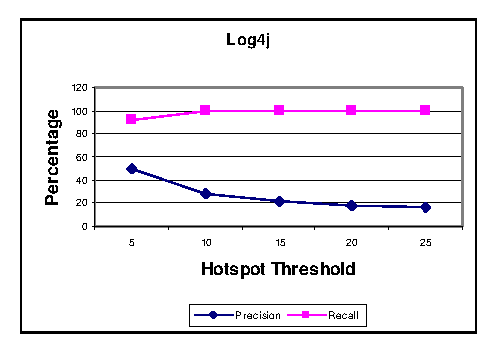
\includegraphics[scale=0.72,clip]{log4j.eps}
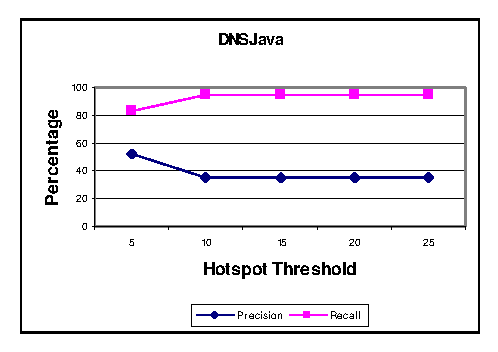
\includegraphics[scale=0.72,clip]{dnsjava.eps}
\caption{\label{fig:precrecall}Precision and Recall for five $HT$ values with JUnit, Log4j, and DNSJava} \vspace{-2.5ex}
\end{figure*}

We next describe our empirical analysis with several $HT$ values and describe
why we use $HT$ of 15\% to identify hotspots. Figure~\ref{fig:precrecall}
shows the results with three subjects and several threshold values ranging from 5\% to 25\%.
With the increase in the threshold value, the precision decreases
and the recall increases. \Fix{Although decrease in the precision is common with 
increase in the threshold value, the figure shows that the precision
decreases rapidly with increase in the threshold value from 5\% to 10\%. 
This observation indicates that many commonly reused API methods (even among the top 10\% 
of ranked API methods detected by SpotWeb based on usage) are not included in the documentation. This phenomenon
shows that the real hotspots of these frameworks are beyond those hotspots
calculated based on the documentation because the documentation
of existing frameworks is often outdated or incomplete.} This evaluation shows the necessity
of an approach such as SpotWeb that can automatically infer hotspots
from the applications that are already reusing the API classes and methods of the input framework.

In our implementation, we used $HT$ as 15\%
as this threshold value has high recall with reasonable precision.
The primary reason for inclining toward a high recall with low precision
is that the framework users would miss few hotspot classes. To alleviate the low precision,
our ranking mechanism helps give higher priority to those
hotspot classes that are described in the documentation compared
to other classes as shown in Table~\ref{tab:hdresults}.
%---------------------------------------------------------------------------
\subsubsection{Comparison with Viljamaa's approach}
We next compare the results of SpotWeb with the results of a previous related approach by Viljamaa~\cite{viljamaa:reverse}
for the JUnit framework. Their approach also recovers the hotspots of a framework
by using the source code of the framework and a set of available example applications. Their approach
uses concept analysis~\cite{ganter:concept} for recovering hotspots of the framework. As both approaches target
a similar problem, we compared the results of SpotWeb for the JUnit framework with the
results of their approach. \Fix{Viljamaa's approach detected a total of 7 classes
as hotspot classes for JUnit framework, whereas SpotWeb detected 14 classes
as hotspot classes. Section~\ref{sec:doccomp} presents the precision
and recall values for SpotWeb with respect to the JUnit documentation.}

SpotWeb detected 5 classes among the 7 classes detected by Viljamaa's approach. The 2 missing classes
are \CodeIn{ExceptionTestCase} and \CodeIn{ActiveTestSuite}. However, both
these classes are not described in the available documentation of JUnit.
SpotWeb is not able to detect these classes because of low 
support among gathered code examples. SpotWeb detected 4 new classes and several
new methods that are not detected by Viljamaa's approach and are described in the documentation. 
For example, classes of JUnit such as \CodeIn{Assert}, \CodeIn{TestResult},
and \CodeIn{TestFailure} (shown in Figure~\ref{fig:hotspotexample}) 
are often used and detected only by SpotWeb. Similarly, for the
\CodeIn{Testcase} class, the \CodeIn{tearDown} method is also often used along with
the \CodeIn{setUp} method. Viljamaa's approach detected only the \CodeIn{setUp} method, whereas
SpotWeb detected both \CodeIn{setUp} and \CodeIn{tearDown} methods as hotspot methods.
These results show that SpotWeb can perform better than Viljamaa's approach.
Furthermore, Viljamaa's approach requires the users to have 
some initial knowledge of the structure and hotspots of the input framework that is being analyzed.
In contrast, our approach does not require the users to have any knowledge regarding the 
input framework.

\section{Threats to Validity}
\label{sec:threats}
The threats to external validity primarily include the degree to
which the subject programs and used CSE are representative of true
practice. The current subjects range from small-scale applications
such as Grappa to large-scale applications such as BCEL and JUNG. In
SpotWeb, we used only one CSE, i.e., Google code search. We plan to
reduce these threats by conducting more experiments on wider types
of subjects and by using other CSEs in future work. The threats to
internal validity are instrumentation effects that can bias our
results. Faults in our SpotWeb prototype might cause such effects
while detecting hotspots and coldspots. To reduce these threats, we
inspected some code examples gathered from the CSE to double check
the metrics computed by SpotWeb for these code examples.\vspace{-1ex}
%------------------------------------------------------------------------
\section {Related Work}
\label{sec:related}
We used CSEs for gathering related code examples in our 
previous approaches called MAPO~\cite{mapo:xie} and PARSEWeb~\cite{thummalapenta07:parseweb}.
With MAPO and PARSEWeb, SpotWeb shares \emph{only} the code downloader component that is used for gathering
related code examples. As each approach targets
a different problem, each approach has different techniques 
in analyzing gathered code examples to address the
challenges of that problem. MAPO and PARSEWeb focus on mining
API usage patterns to assist programmers to write effective API client code.
Given an API method, MAPO identifies the frequent usage patterns of that API method from
gathered code examples. PARSEWeb analyzes each gathered code example and builds
a CFG, which includes only method-invocation nodes, and captures sequences
that serve as solutions for the queries of the form ``Source object type $\rightarrow$ Destination object type''.
The SpotWeb approach is significantly different from these approaches as SpotWeb targets at capturing
\emph{UsageMetrics} of classes and methods of a given input framework and uses
these metrics to detect hotspots and coldspots.

An approach by Viljamaa~\cite{viljamaa:reverse} also recovers the hotspots of a framework
by using the source code of the input framework and a set of available example applications. Their approach
uses concept analysis~\cite{ganter:concept} for uncovering hotspots of the framework. One major
problem with their approach is that applying concept analysis to the entire input source code
can result in a huge pattern that is not useful in practice. To
address the preceding problem, their approach 
suggests to select only those program elements 
that are relevant to the hotspot \emph{h} at hand. Therefore, their
approach requires the users to have some initial knowledge of the structure
and hotspots of the framework under analysis. In contrast,
our approach uses simple statistical analysis and can handle an entire input
framework. Furthermore, SpotWeb does not require
the users to have any knowledge of the input framework. Finally,
our approach performs better than their approach as shown in our evaluation.

Mendonca et al.~\cite{mendoca:instantiation} proposed an approach to
assist framework instantiation and to understand the intricate
details surrounding the framework design.
However, their approach requires framework developers to
manually specify the framework design in a specific process
language, called Reuse Definition Language, proposed by their approach.

Holmes and Walker~\cite{holmes:apiusage} proposed an approach 
that quantitatively determines how existing APIs are used. Their approach
gathers a few applications that already reuse those existing APIs
and computes metrics to detect how existing APIs are used by those applications.
SpotWeb differs from their approach in three main aspects. First, their approach 
expects the framework users to have knowledge 
of the APIs of the framework. Therefore, their approach is mainly useful to users who are already
familiar with those framework APIs. Second, their approach presents only the
number of times that the APIs are reused. Third, their approach computes metrics
from a limited data scope. In contrast, SpotWeb does not require the users
to have the knowledge of APIs of the input framework and presents information
in a more comprehensive form through templates and hooks.

Baxter et al.~\cite{baxter:shape} proposed an approach to discover
the structure of Java programs and the way that the classes relate
to each other through inheritance and composition. Their study is
useful for framework developers who can evaluate the structural
features of their own programming practice and optimize their
performance. In contrast, SpotWeb is useful for framework users
in effectively reusing the APIs of a framework.

\section {Conclusion}
\label {sec:conclusion}

In this paper, we proposed an approach called SpotWeb that 
assists software developers in reusing API classes and methods of an existing framework
by detecting hotspots and coldspots of the framework. \Comment{Hotspots can serve
as starting points for reusing the framework, whereas coldspots serve as caveats as there can 
be difficulties in finding related code examples.}
SpotWeb addresses major problems faced by previous 
related approaches by not requiring any additional effort
from the developers and by collecting relevant code examples through
a code search engine. In our evaluation, we found that often classes
of existing frameworks are either reused heavily or never reused.
We also showed that the detected hotspots are 
indeed useful in helping effective framework reuse 
and showed that SpotWeb performs better than an earlier related
approach. In future work, we plan to explore other applications
of hotspots such as prioritization of bug reports based on hotspots.

\vfill\eject
\section*{Acknowledgments}

This work is supported in part by NSF grants CNS-0720641 and
CCF-0725190, and Army Research Office grant W911NF-07-1-0431.

\bibliographystyle{IEEEtran}

% Generated by IEEEtran.bst, version: 1.12 (2007/01/11)
\begin{thebibliography}{10}
\providecommand{\url}[1]{#1}
\csname url@samestyle\endcsname
\providecommand{\newblock}{\relax}
\providecommand{\bibinfo}[2]{#2}
\providecommand{\BIBentrySTDinterwordspacing}{\spaceskip=0pt\relax}
\providecommand{\BIBentryALTinterwordstretchfactor}{4}
\providecommand{\BIBentryALTinterwordspacing}{\spaceskip=\fontdimen2\font plus
\BIBentryALTinterwordstretchfactor\fontdimen3\font minus
  \fontdimen4\font\relax}
\providecommand{\BIBforeignlanguage}[2]{{%
\expandafter\ifx\csname l@#1\endcsname\relax
\typeout{** WARNING: IEEEtran.bst: No hyphenation pattern has been}%
\typeout{** loaded for the language `#1'. Using the pattern for}%
\typeout{** the default language instead.}%
\else
\language=\csname l@#1\endcsname
\fi
#2}}
\providecommand{\BIBdecl}{\relax}
\BIBdecl

\bibitem{document:leth}
T.~C. Lethbridge, J.~Singer, and A.~Forward, ``{How Software Engineers use
  Documentation: The State of the Practice},'' in \emph{IEEE Software},
  vol.~20, no.~6.\hskip 1em plus 0.5em minus 0.4em\relax Los Alamitos, CA, USA:
  IEEE Computer Society Press, 2003, pp. 35--39.

\bibitem{pree:metapatterns}
W.~Pree, ``{Meta Patterns - A Means For Capturing the Essentials of Reusable
  Object-Oriented Design},'' in \emph{Proceedings of the 8th European
  Conference on Object-Oriented Programming (ECOOP)}.\hskip 1em plus 0.5em
  minus 0.4em\relax London, UK: Springer-Verlag, 1994, pp. 150--162.

\bibitem{martin:open}
R.~C. Martin, ``{The Open Closed Principle},'' \emph{{j-C-PLUS-PLUS-REPORT}},
  vol.~8, no.~1, pp. 37--43, 1996.

\bibitem{thummalapenta08:spotweb}
S.~Thummalapenta and T.~Xie, ``{{SpotWeb}: Detecting Framework Hotspots via
  Mining Open Source Repositories on the Web},'' in \emph{Proceedings of the
  2008 International Workshop on Mining Software Repositories (MSR)}.\hskip 1em
  plus 0.5em minus 0.4em\relax New York, NY, USA: ACM, 2008, pp. 109--112.

\bibitem{viljamaa:reverse}
J.~Viljamaa, ``{Reverse Engineering Framework Reuse Interfaces},'' in
  \emph{Proceedings of the 9th European Software Engineering Conference held
  jointly with 11th ACM SIGSOFT International Symposium on Foundations of
  Software Engineering (ESEC/FSE)}.\hskip 1em plus 0.5em minus 0.4em\relax New
  York, NY, USA: ACM, 2003, pp. 217--226.

\bibitem{JUNIT}
``{JUnit},'' 2001, \url{http://www.junit.org}.

\bibitem{GCSE}
``{Google Code Search},'' 2006, \url{http://www.google.com/codesearch}.

\bibitem{thummalapenta07:parseweb}
S.~Thummalapenta and T.~Xie, ``{PARSEWeb}: {A Programmer Assistant for Reusing
  Open Source Code on the Web},'' in \emph{Proceedings of the 22nd IEEE/ACM
  International Conference on Automated Software Engineering (ASE)}.\hskip 1em
  plus 0.5em minus 0.4em\relax New York, NY, USA: ACM, 2007, pp. 204--213.

\bibitem{ganter:concept}
B.~Ganter and R.~Wille, \emph{{Formal Concept Analysis: Mathematical
  Foundations}}.\hskip 1em plus 0.5em minus 0.4em\relax Secaucus, NJ, USA:
  Springer-Verlag New York, Inc., 1997, translator-C. Franzke.

\bibitem{mapo:xie}
T.~Xie and J.~Pei, ``{MAPO: Mining API Usages from Open Source Repositories},''
  in \emph{Proceedings of the 2006 International Workshop on Mining Software
  Repositories (MSR)}.\hskip 1em plus 0.5em minus 0.4em\relax New York, NY,
  USA: ACM, 2006, pp. 54--57.

\bibitem{mendoca:instantiation}
M.~Mendonca, P.~Alencar, T.~Oliveira, and D.~Cowan, ``{A}ssisting
  Aspect-Oriented Framework Instantiation: Towards Modeling, Transformation and
  Tool Support,'' in \emph{Companion to the 20th Annual ACM SIGPLAN Conference
  on Object-Oriented Programming, Systems, Languages, and Applications
  (OOPSLA)}.\hskip 1em plus 0.5em minus 0.4em\relax New York, NY, USA: ACM,
  2005, pp. 94--95.

\bibitem{holmes:apiusage}
R.~Holmes and R.~J. Walker, ``{Informing {Eclipse API} Production and
  Consumption},'' in \emph{Proceedings of the 2007 OOPSLA Workshop on Eclipse
  Technology eXchange (ETX)}, 2007, pp. 70--74.

\bibitem{baxter:shape}
G.~Baxter, M.~Frean, J.~Noble, M.~Rickerby, H.~Smith, M.~Visser, H.~Melton, and
  E.~Tempero, ``{U}nderstanding the Shape of {J}ava Software,'' \emph{SIGPLAN
  Not.}, vol.~41, no.~10, pp. 397--412, 2006.

\end{thebibliography}

\end{document}
